\documentclass[11pt,a4paper]{article}
\usepackage[T1]{fontenc}
\usepackage{lmodern}
\usepackage[a4paper,top=24mm,bottom=24mm,left=22mm,right=22mm]{geometry}
\usepackage{graphicx}
\usepackage{booktabs}
\usepackage{tabularx}
\usepackage{array}
\usepackage[table]{xcolor}
\usepackage{enumitem}
\usepackage{titlesec}
\usepackage{fancyhdr}
\usepackage{caption}
\usepackage{float}
\usepackage{amsmath}
\usepackage[colorlinks=true,linkcolor=osdagdark,urlcolor=osdagdark]{hyperref}

\definecolor{osdag}{HTML}{91B014}
\definecolor{osdagdark}{HTML}{4F6608}
\definecolor{codebg}{HTML}{F4F7EA}
\titleformat{\section}{\large\sffamily\bfseries\color{osdagdark}}{\thesection}{0.7em}{}
\titleformat{\subsection}{\normalsize\sffamily\bfseries\color{osdagdark}}{\thesubsection}{0.7em}{}
\captionsetup{font=small,labelfont={bf,color=osdagdark}}
\setlist{itemsep=2pt,topsep=3pt}
\setlength{\parskip}{4pt}\setlength{\parindent}{0pt}
\newcommand{\code}[1]{\texttt{\small #1}}
\newcolumntype{Y}{>{\raggedright\arraybackslash}X}
\pagestyle{fancy}\fancyhf{}
\fancyhead[L]{\small\sffamily OsdagBridge Report Generator --- Technical Changes}
\fancyhead[R]{\small\sffamily Screening Task}
\fancyfoot[C]{\small\thepage}
\renewcommand{\headrule}{{\color{osdag}\hrule height 0.8pt}}

\begin{document}

\begin{center}
{\color{osdag}\rule{\linewidth}{1.2pt}}\\[8pt]
{\LARGE\sffamily\bfseries OsdagBridge Design Report Generator}\\[4pt]
{\Large\sffamily Refactoring \& Enhancements --- Technical Changes Report}\\[10pt]
{\normalsize Shreyash Trivedi \quad$\cdot$\quad FOSSEE Osdag Screening Task \quad$\cdot$\quad 13 November 2026}\\[4pt]
{\small Code: \url{https://github.com/shreyashtrivedi/OsdagBridge/tree/report-refactor}}\\[6pt]
{\color{osdag}\rule{\linewidth}{1.2pt}}
\end{center}

\section{Summary}

The report generator (\code{src/osdagbridge/core/reports/}) was refactored so that every table is
built through one PyLaTeX-based table builder and every visual attribute comes from one style
module. All six items of the task are implemented and verified on the same design data before and
after the change (Table~\ref{tab:summary}). While testing, several correctness bugs in the existing
report were found and fixed; they are listed in Section~\ref{sec:fixes}.

\begin{table}[H]
\centering\small
\caption{Task requirements and where they are addressed}\label{tab:summary}
\begin{tabularx}{\linewidth}{>{\raggedright\arraybackslash}p{3.6cm}Y>{\raggedright\arraybackslash}p{3.4cm}}
\toprule
\textbf{Requirement} & \textbf{Result} & \textbf{Main files}\\
\midrule
1. Repeated table headers & Caption + column header repeat on every page of every multi-page table (\code{\textbackslash endfirsthead}/\code{\textbackslash endhead}); short tables never split. & \code{report\_tables.py}\\
2. Footer overlap \& spacing & Row groups (e.g.\ girder ``G4'') can no longer split or bleed into the footer; footer lives entirely in the bottom margin; page-bottom thresholds. & \code{report\_tables.py}, \code{styles.py}\\
3. Load tables & Separate vehicle live-load table (as per the example: total load, impact factor, braking considered / value / eccentricity) and footway table; only vehicles selected in the Loading tab. & \code{chap3.py}\\
4. UR charts & Section 5.5: governing UR per element and UR per check, red dashed UR = 1.0 line. & \code{report\_charts.py}, \code{chap5.py}\\
5. Material charts & Chapter 7: steel tonnage (girders, cross bracing, end diaphragms) and concrete m$^3$ vs.\ reinforcement MT, embedded via PyLaTeX \code{Figure}. & \code{report\_charts.py}, \code{chap7.py}, \code{boq\_generator.py}\\
6. Central style system & \code{styles.py} is the single source of truth for page geometry, colours, fonts, table padding, header/footer and chart style. & \code{styles.py}\\
\bottomrule
\end{tabularx}
\end{table}

\textbf{Measured effect} (same design data, 30\,m span, 5 girders): the report shrank from 56 to 46 pages;
hidden LaTeX errors went from 140 to 0 (the original compiles in \code{nonstopmode}, which hides them);
no overfull boxes; ``Page X of Y'' is now correct.

\section{Architecture}

The existing chapters assembled raw LaTeX strings. A full rewrite into a PyLaTeX \code{Document}
tree would have touched about 4{,}400 lines of engineering data logic, so a \emph{hybrid} design was
chosen: the data extraction in each chapter is kept, and only the \emph{presentation} is moved into three
new modules that all chapters import.

\begin{center}\small
\begin{tabular}{l}
\code{report\_generator.py} \quad orchestration, preamble, \code{ReportDataBridge}\\
\quad $\downarrow$ calls \code{executive\_summary}, \code{chap1} \dots\ \code{chap9}\\
\quad\quad $\downarrow$ every table \quad $\rightarrow$ \code{report\_tables.ReportTable} \quad (PyLaTeX \code{LongTable} / \code{Tabular})\\
\quad\quad $\downarrow$ every chart \quad $\rightarrow$ \code{report\_charts} \quad (matplotlib PNG $\rightarrow$ PyLaTeX \code{Figure})\\
\quad\quad $\downarrow$ every length, colour, font \quad $\rightarrow$ \code{styles}\\
\end{tabular}
\end{center}

\textbf{Why hybrid:} the engineering values in the report are unchanged (lower regression risk), while all
layout behaviour is concentrated in one tested place. A chapter now describes \emph{what} a table contains,
e.g.\ \code{t.group("G1", rows)}, and the builder decides \emph{how} it is typeset and broken across pages.

\section{Requirement-by-requirement changes}

\subsection{Repeated table headers across page breaks}
\code{ReportTable} builds every multi-page table as a PyLaTeX \code{LongTable}:
\begin{itemize}
\item caption + header row in \code{\textbackslash endfirsthead}; a ``(continued)'' caption + the same header in
\code{\textbackslash endhead} (PyLaTeX \code{end\_table\_header()}), so the header appears on every page;
\item ``continued on next page'' in \code{\textbackslash endfoot}; the table note in \code{\textbackslash endlastfoot},
so a note can never be orphaned on the next page;
\item tables with $\leq 12$ rows are emitted as a PyLaTeX \code{Tabular} inside an unbreakable minipage and
move to the next page as a whole instead of splitting;
\item column widths are relative weights converted to \code{\textbackslash linewidth}-based dimensions, so no
table can exceed the text width whatever the page geometry.
\end{itemize}
The one pre-existing table with repeated headers (Table 4.1, two-level header) is kept and now uses the same builder.

\begin{figure}[H]
\centering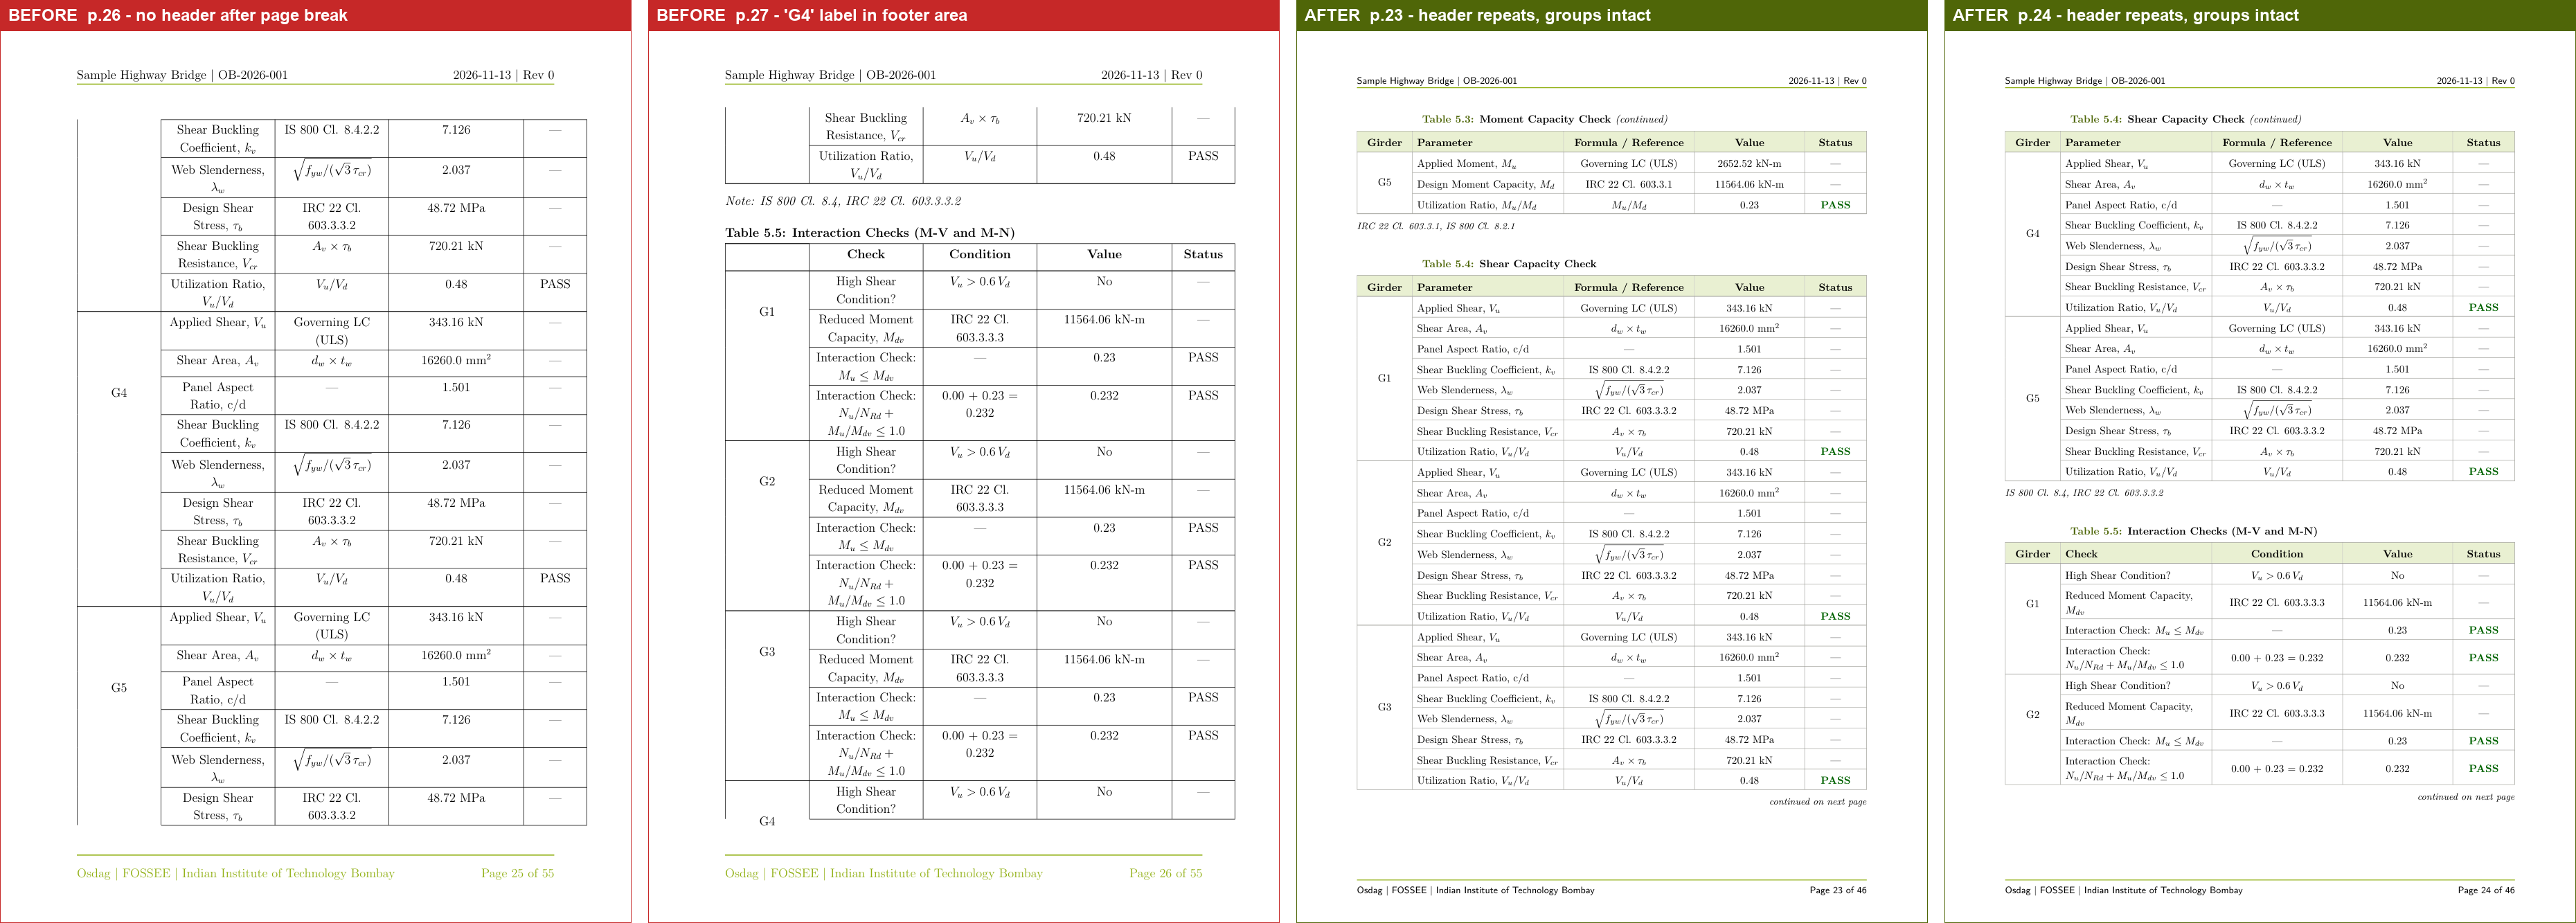
\includegraphics[width=\linewidth]{images/cmp_headers_footer.png}
\caption{Before: continuation pages have no header and the ``G4'' label is pushed below the table into the
footer area. After: header repeats and each girder group stays on one page.}
\end{figure}

\subsection{Layout, footer overlap and vertical spacing}
Three root causes were identified by testing against the bundled TeX distribution:
\begin{enumerate}
\item \textbf{Split multirow groups.} A girder's 13-row block was allowed to break across pages, so the
\code{\textbackslash multirow} label (``G4'') was centred over rows on the next page and printed in the footer.
Group rows are now bound with \code{\textbackslash nopagebreak}.
\item \textbf{\code{\textbackslash cline} is a breakpoint.} \code{colortbl}'s \code{\textbackslash cline} ends with
\code{\textbackslash noalign\{\textbackslash vskip-\textbackslash arrayrulewidth\}}; that skip follows a box and is
a legal page break, so penalties could not bind a group. A non-breaking variant \code{\textbackslash nbcline} is
defined in the preamble and used inside groups.
\item \textbf{Orphaned headers.} A \code{\textbackslash needspace} placed directly before
\code{\textbackslash begin\{longtable\}} lets the break fall \emph{inside} the table (only the footer is left on the
old page). It was removed; longtable's own start check now measures header + footer + the whole first group.
\end{enumerate}
The footer is a single box (software-default note, rule, footer text) placed in the bottom margin with
explicit \code{footskip}/\code{bottom} geometry, replacing the old negative \code{\textbackslash vspace} hack in
\code{\textbackslash footrule}. Uniform cell padding comes from \code{\textbackslash arraystretch} and
\code{\textbackslash extrarowheight} instead of per-row \code{\textbackslash\textbackslash[6pt]}.

\subsection{Load and geometry tables (Chapter 3)}
The merged ``Live Loads (LL)'' table was split into:
\begin{itemize}
\item \textbf{Vehicle live loads} --- one row per vehicle ticked in the Loading tab, columns exactly as the
reference example: \emph{Vehicle $|$ Total Load (kN) $|$ Impact Factor $|$ Braking Load: Considered? / Value / Eccentricity}.
Total loads come from the IRC~6 vehicle definitions in \code{irc6\_2017.py}; impact factors use the same IRC~6
functions as the analysis; ``Considered?'' follows the app's rules (vehicle trains yes, Class~SV per its own
braking check box, 70R bogie and fatigue vehicle no); eccentricity is the user's ``Eccentricity from top of deck''
input. Centrifugal force (IRC~6 Cl.~212) is reported as not applicable to a straight span.
\item \textbf{Footway live load} --- configuration, width, pressure basis, design intensity, line load per footpath
and total load; replaced by a one-line note when the bridge has no footpath.
\end{itemize}
The wind and seismic tables now show the computed $V_z$, $P_z$, $Z$, $S_a/g$, $A_h$, $A_v$ (previously computed
but never printed). Permanent, live and environmental loads are grouped under their own sections.

\begin{figure}[H]
\centering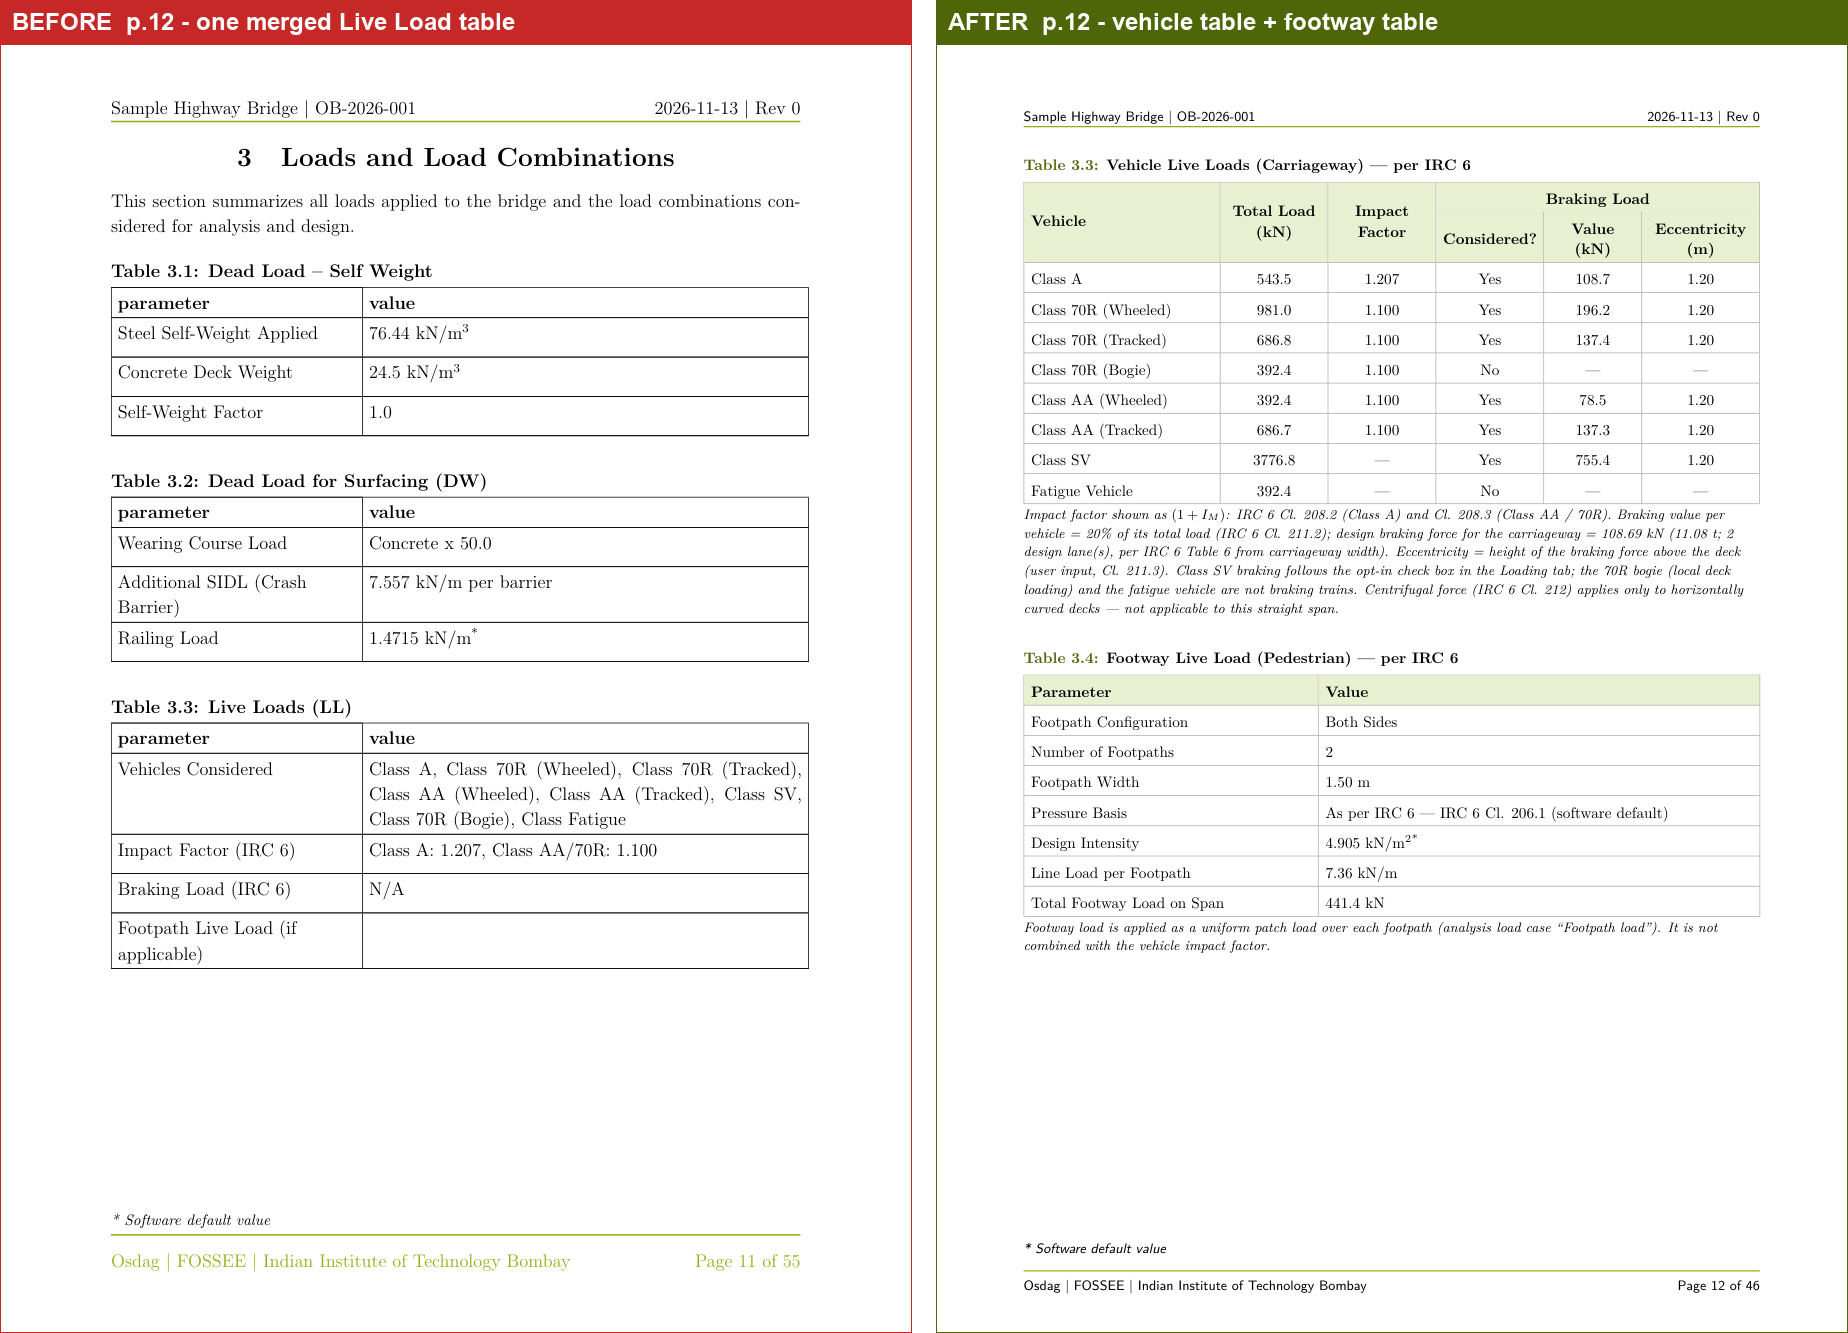
\includegraphics[width=0.82\linewidth]{images/cmp_live_loads.png}
\caption{Chapter 3 live loads before and after.}
\end{figure}

\subsection{Utilization ratio summary charts (Section 5.5)}
The overall summary function now returns, together with the table, the numeric UR of every check grouped by
element (steel plate girders, concrete deck slab, cross bracing, end diaphragms). The \emph{same numbers}
drive the table and two charts, so they cannot disagree:
\begin{itemize}
\item governing UR per element; and UR per check, one panel per element on a shared UR scale;
\item y-axis = UR, red dashed horizontal line at UR = 1.0; bars above the line are red and labelled ``FAIL''
(status is never conveyed by colour alone); elements without results are shown as ``n/a'' rather than omitted.
\end{itemize}

\begin{figure}[H]
\centering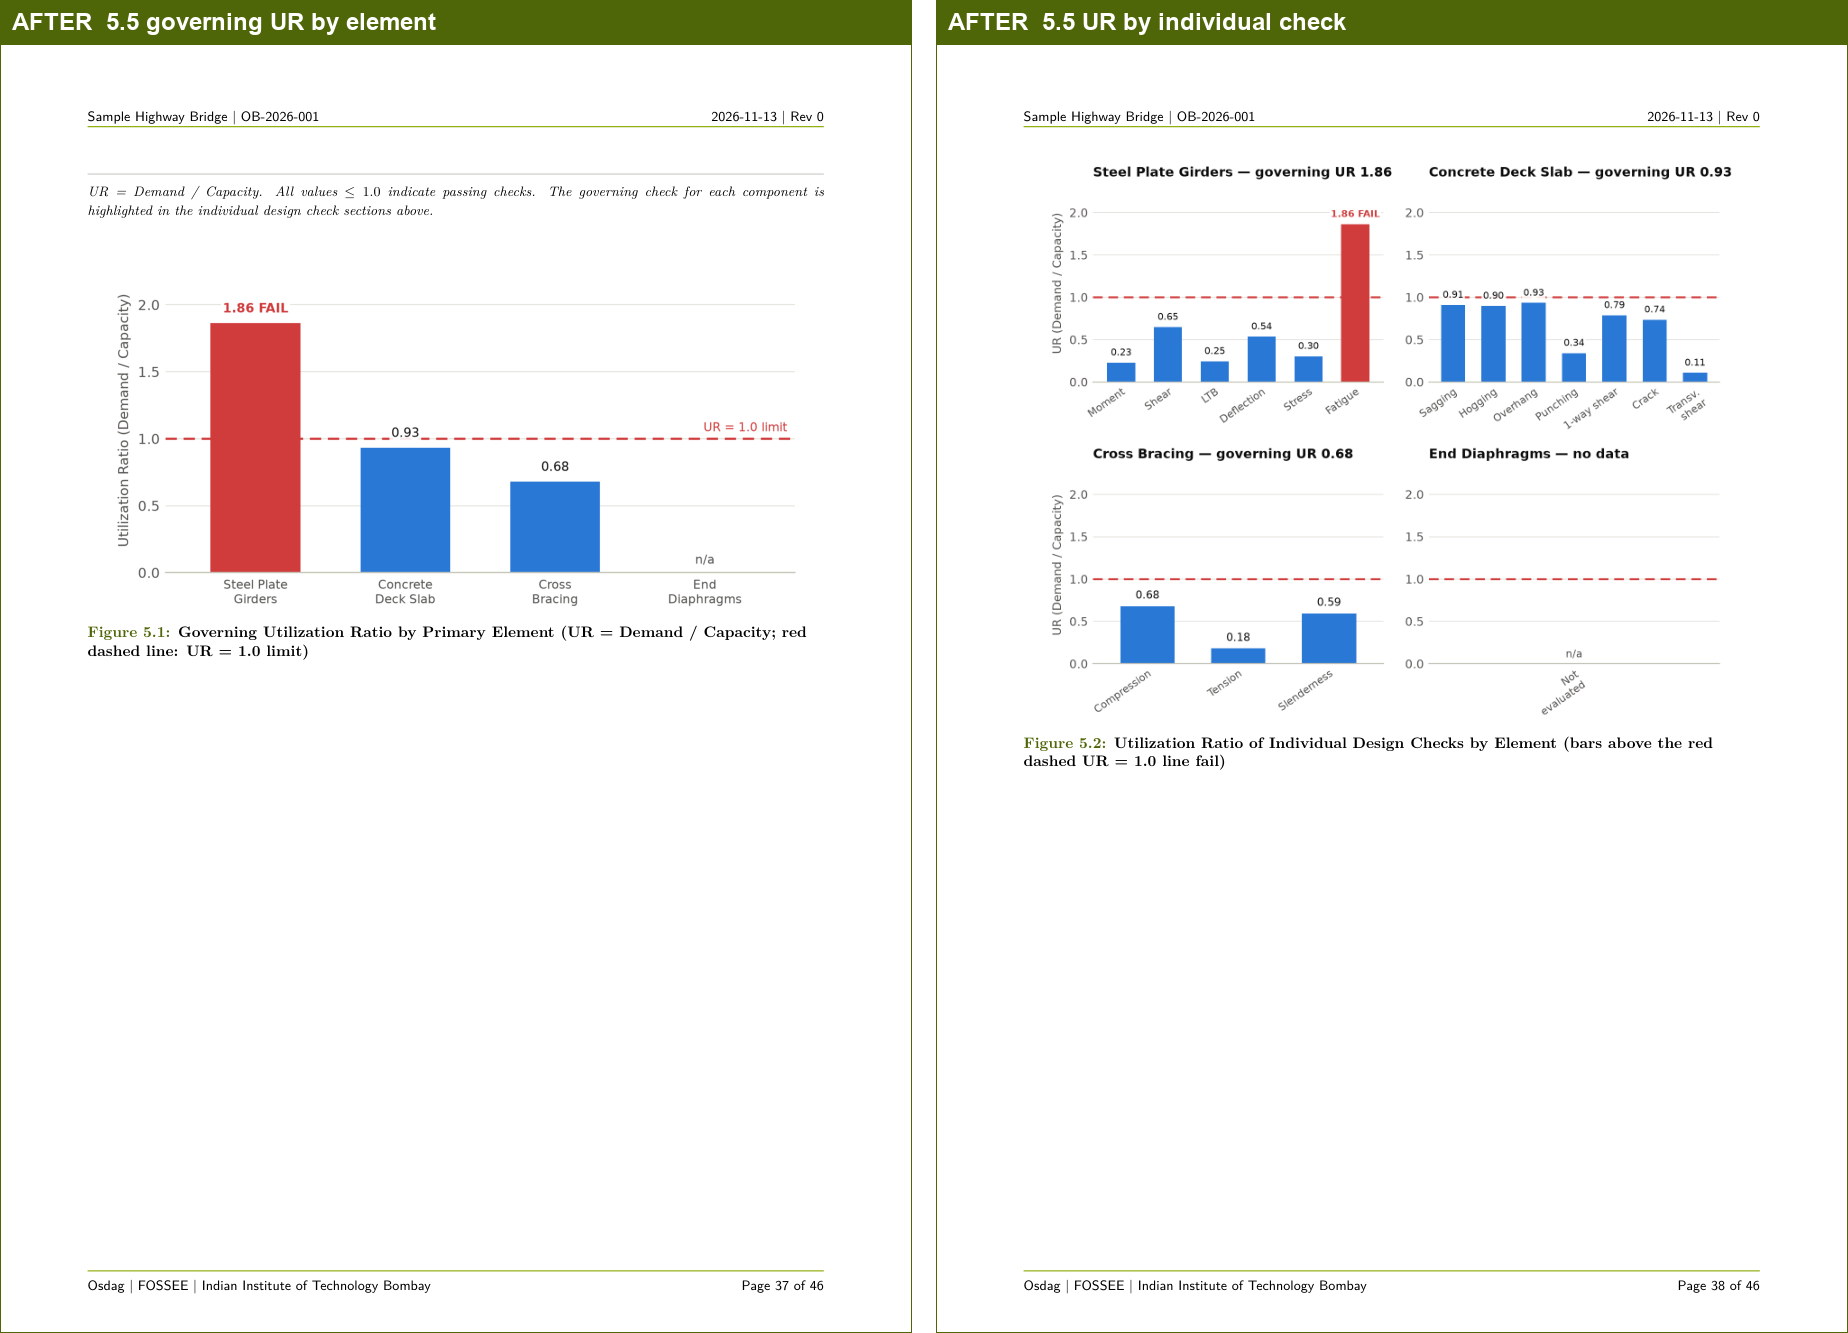
\includegraphics[width=0.82\linewidth]{images/after_ur_charts.png}
\caption{New Section 5.5 charts (fatigue governs the girders at UR 1.86 for the sample design).}
\end{figure}

\subsection{Material quantity charts (Chapter 7)}
\code{boq\_generator.py} gained an end-diaphragm take-off (both supports; bracing-type diaphragms use diagonals +
chords, rolled/welded types one beam per bay). Table 7.1 shows the new row and a structural-steel total. Two charts
are written to the report's temporary image folder and embedded with PyLaTeX \code{Figure}: steel tonnage by element,
and concrete volume (m$^3$) beside reinforcement weight (MT) as two panels with their own axes (a dual-axis chart would
make the two scales look comparable); the caption also gives the deck reinforcement density.

\begin{figure}[H]
\centering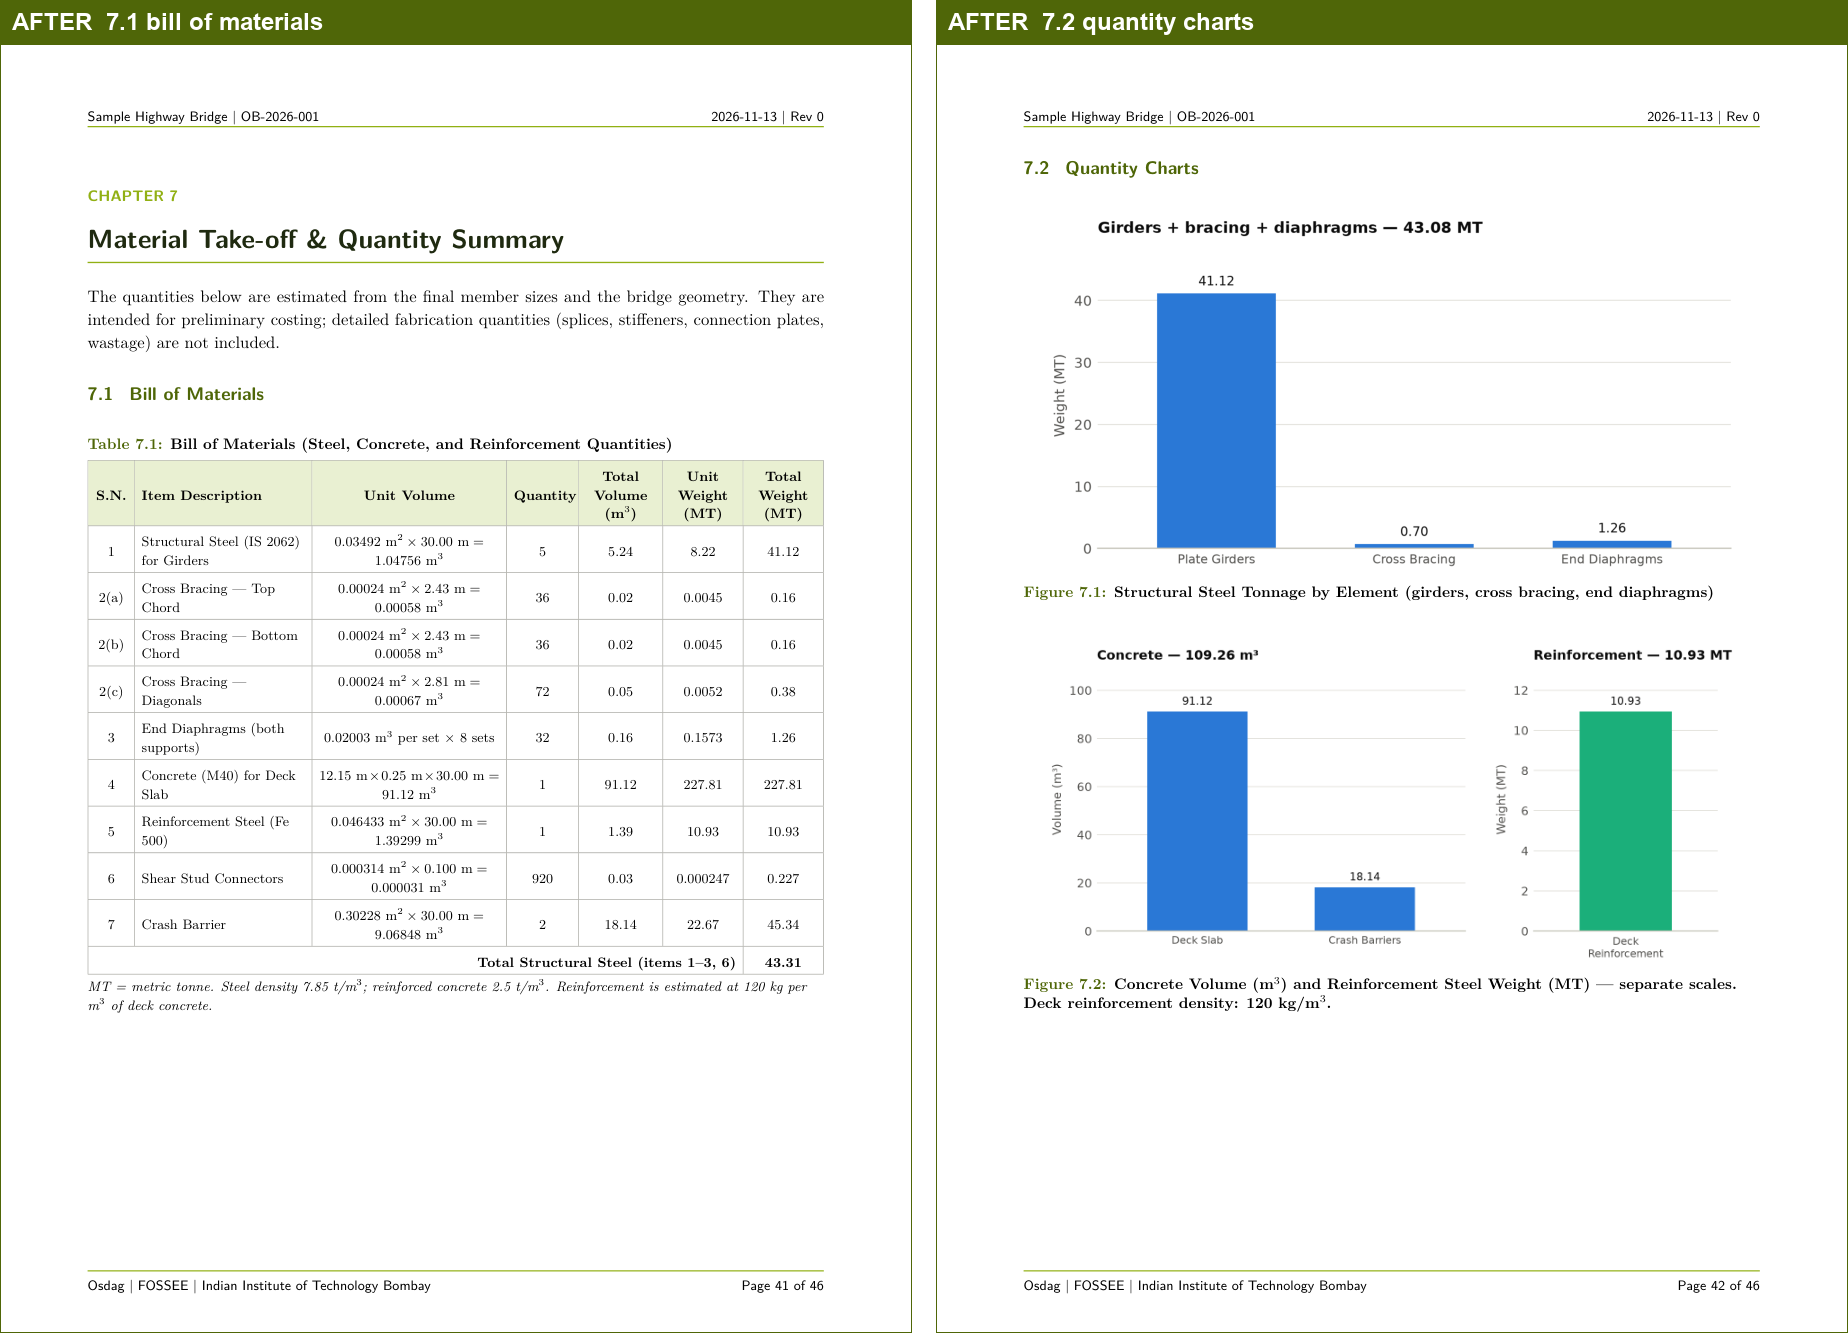
\includegraphics[width=0.82\linewidth]{images/after_quantity_charts.png}
\caption{Bill of materials and quantity charts.}
\end{figure}

\subsection{Centralized formatting \& style system}
\code{styles.py} is the only place where layout and visual attributes are defined. Chapters import helpers
from it and never hard-code lengths, colours or fonts.

\begin{table}[H]
\centering\small
\caption{Structure of \code{styles.py}}
\begin{tabularx}{\linewidth}{>{\raggedright\arraybackslash}p{3.2cm}Y}
\toprule
\textbf{Item} & \textbf{Contents}\\
\midrule
\code{PAGE} & paper, font size, margins, header height/separation, footskip, line spacing\\
\code{COLORS} & brand green, heading ink, table header / section fills, rule colour, PASS/WARN/FAIL text colours (all $\geq$4.5:1 contrast)\\
\code{TYPOGRAPHY} & chapter/section heading styles, caption style, note font\\
\code{TABLE} & fonts, cell padding, row stretch, rule width, space before/after, keep-together and page-bottom thresholds, ``continued'' texts\\
\code{FIGURE}, \code{TITLE\_PAGE} & default widths, placement, placeholder style; title-page layout\\
\code{CHART} & matplotlib DPI, sizes, fonts, series / fail / limit-line colours, line style\\
\code{HEADER\_FOOTER} & running header/footer text, rule colour and width, software-default note\\
\code{status()}, \code{ur\_value()}, \code{note()} & uniform PASS/WARN/FAIL badges, UR formatting (red when $>1$), notes\\
\code{build\_preamble()} & generates the whole LaTeX preamble from the dictionaries above\\
\bottomrule
\end{tabularx}
\end{table}

Changing, for example, \code{COLORS["tblHeaderBg"]} or \code{TABLE["row\_stretch"]} restyles every table in the
report; changing \code{PAGE} margins reflows every table because widths are relative.

\section{Files changed}

\begin{table}[H]
\centering\small
\begin{tabularx}{\linewidth}{>{\raggedright\arraybackslash}p{5.6cm}Y}
\toprule
\textbf{File} & \textbf{Change}\\
\midrule
\code{reports/styles.py} \emph{(new)} & central style configuration and preamble builder\\
\code{reports/report\_tables.py} \emph{(new)} & PyLaTeX table builder (\code{ReportTable}, \code{kv\_table}, \code{multicol})\\
\code{reports/report\_charts.py} \emph{(new)} & UR and quantity charts, PyLaTeX \code{Figure} embedding\\
\code{reports/report\_generator.py} & preamble/title page/TOC via styles; end-diaphragm view in \code{ReportDataBridge}; chart folder; 3 LaTeX passes\\
\code{reports/report\_utils.py} & unicode-safe escaping, float formatting, shared placeholder box\\
\code{reports/executive\_summary.py},\newline \code{reports/chap1}--\code{chap8} & all tables moved to the builder; chapter-specific changes above\\
\code{boq/boq\_generator.py} & end-diaphragm quantities\\
\code{utils/codes/irc6\_2017.py} & braking force: \code{NameError} for 1--2 lanes, N$\to$tonne unit fix\\
\code{tools/report\_preview.py} \emph{(new)} & headless report preview / before--after reproduction\\
\code{environment.yml}, \code{pyproject.toml} & \code{pylatex} dependency\\
\bottomrule
\end{tabularx}
\end{table}

\section{Additional fixes and polish}\label{sec:fixes}
\begin{itemize}
\item \textbf{End diaphragm tables showed cross-bracing data.} Section 5.4 reused the cross-bracing rows
(e.g.\ ``40\,x\,40\,x\,3'' instead of the actual IS\,100\,x\,100\,x\,10). \code{ReportDataBridge} now has an
end-diaphragm view; when the analysis returns no diaphragm forces the checks are marked ``not evaluated'' instead of
borrowing other members' results (Figure~\ref{fig:ed}).
\item \textbf{Page X of Y} was one short: the \code{titlepage} environment reset the counter and two LaTeX passes
were not enough once the TOC shifts pagination. Fixed (plain title page, three passes).
\item \textbf{140 hidden LaTeX errors} (longtable captions without \code{\textbackslash\textbackslash},
unescaped $\leq$/$\geq$ in check names, unclosed \code{\textbackslash begingroup}, column-count mismatches) $\rightarrow$ 0.
\item Braking force printed ``N/A'' (\code{NameError}); after that fix the function returned newtons labelled as tonnes --- both fixed (108.7\,kN for 2 lanes).
\item Floating-point noise (``12.149999999999999 m'') trimmed; units added where missing.
\item Table 4.2 (support reactions) was three empty rows; it now lists the envelope and absolute governing reactions.
\item Transverse shear is included in the overall summary; Executive Summary tables are numbered ES.1, ES.2.
\item Visual polish: Latin Modern text with sans-serif headings, ``CHAPTER n'' labels with a green rule, shaded table
headers, light grid rules, colour-coded bold PASS/WARN/FAIL, UR $>1$ in red, dotted TOC leaders, consistent figure
placeholders that never overflow the margin.
\item Environment note: Osdag's section database (\code{Intg\_osdag.sqlite}) is only built when the Osdag GUI is
started; if it is empty, cross-bracing design returns nothing. \code{tools/report\_preview.py} initialises it.
\end{itemize}

\begin{figure}[H]
\centering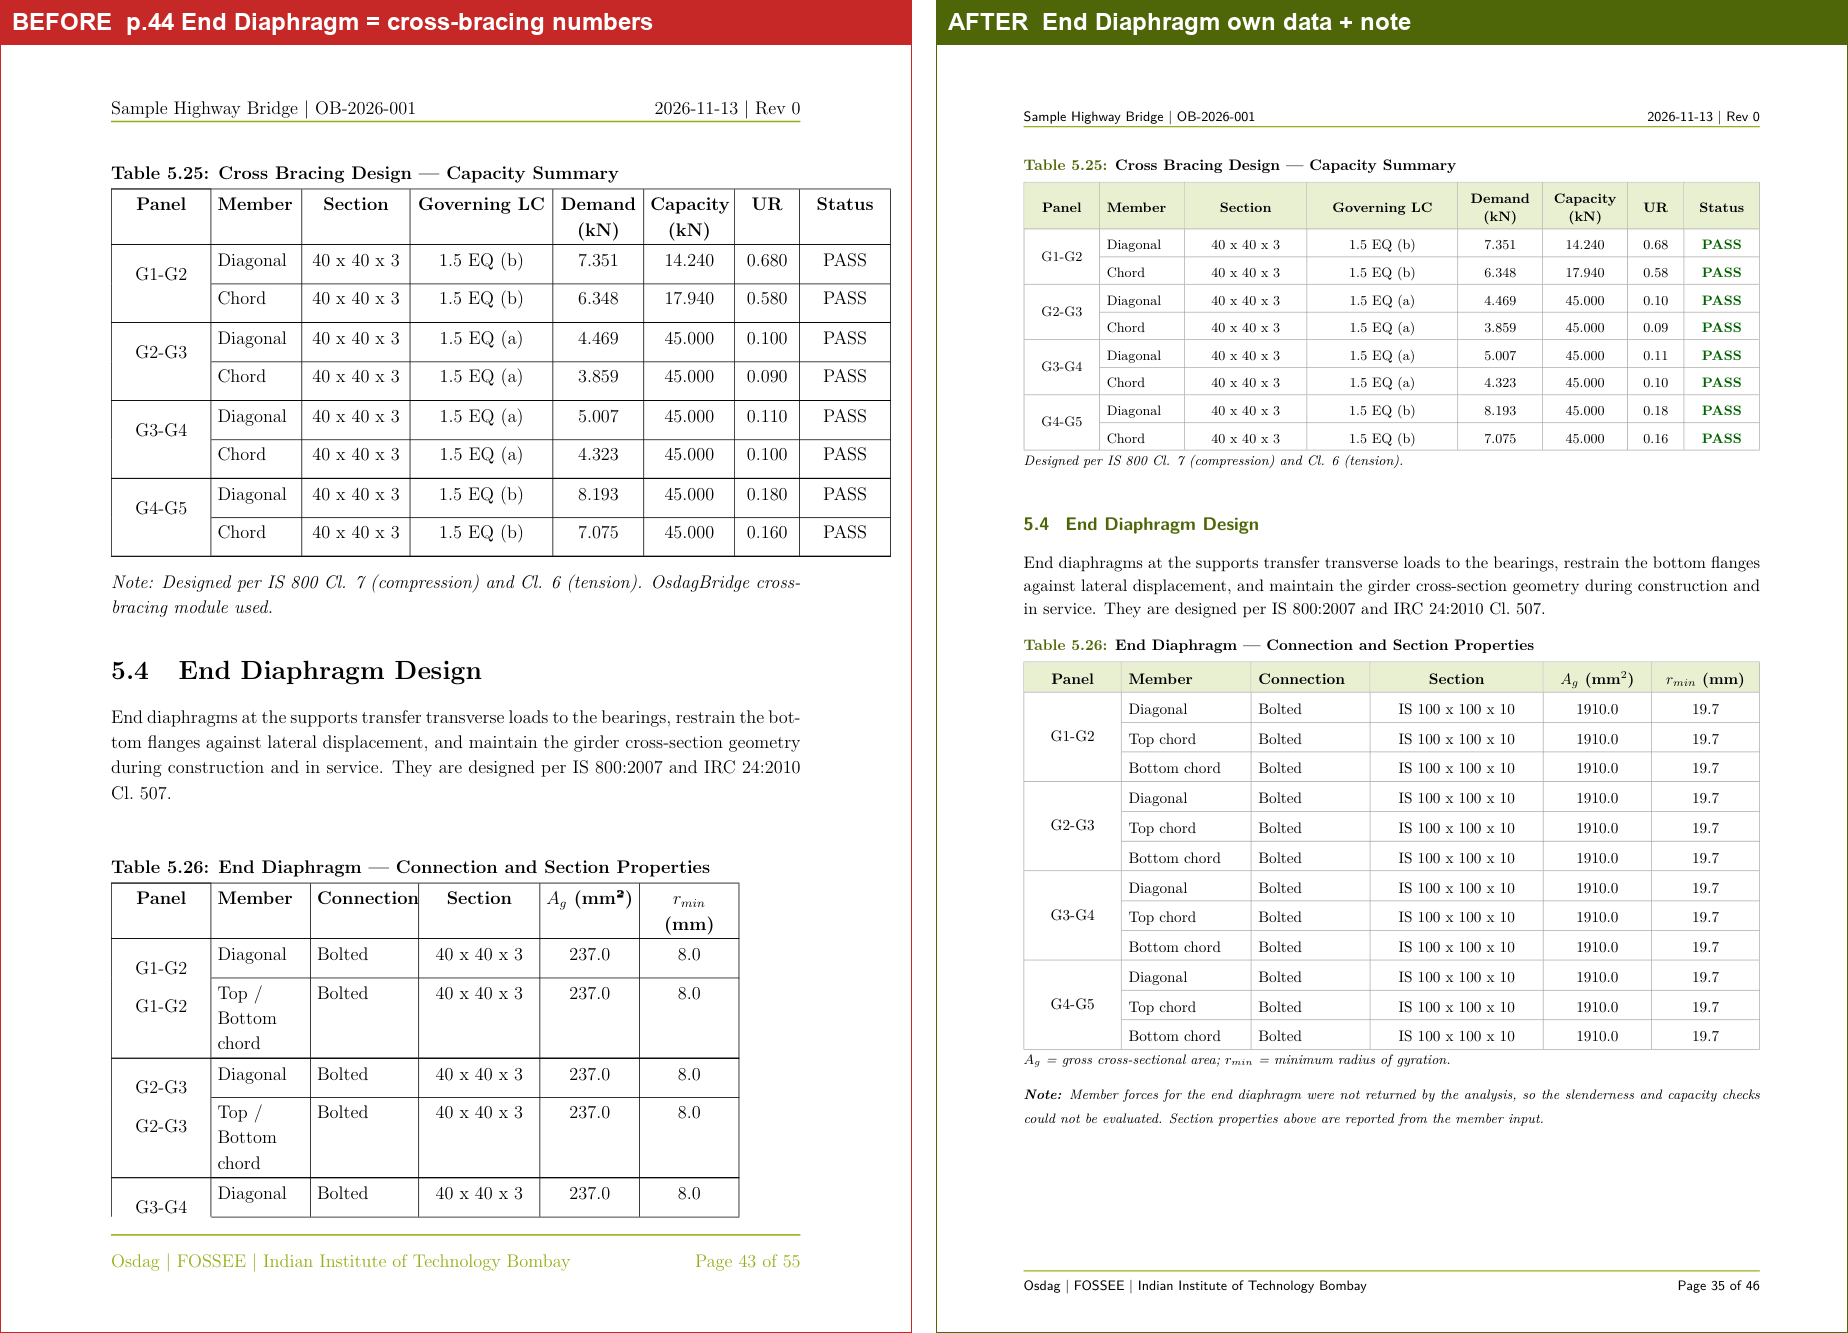
\includegraphics[width=0.82\linewidth]{images/cmp_end_diaphragm.png}
\caption{End diaphragm section: before (cross-bracing numbers) and after (its own section data).}\label{fig:ed}
\end{figure}

\begin{figure}[H]
\centering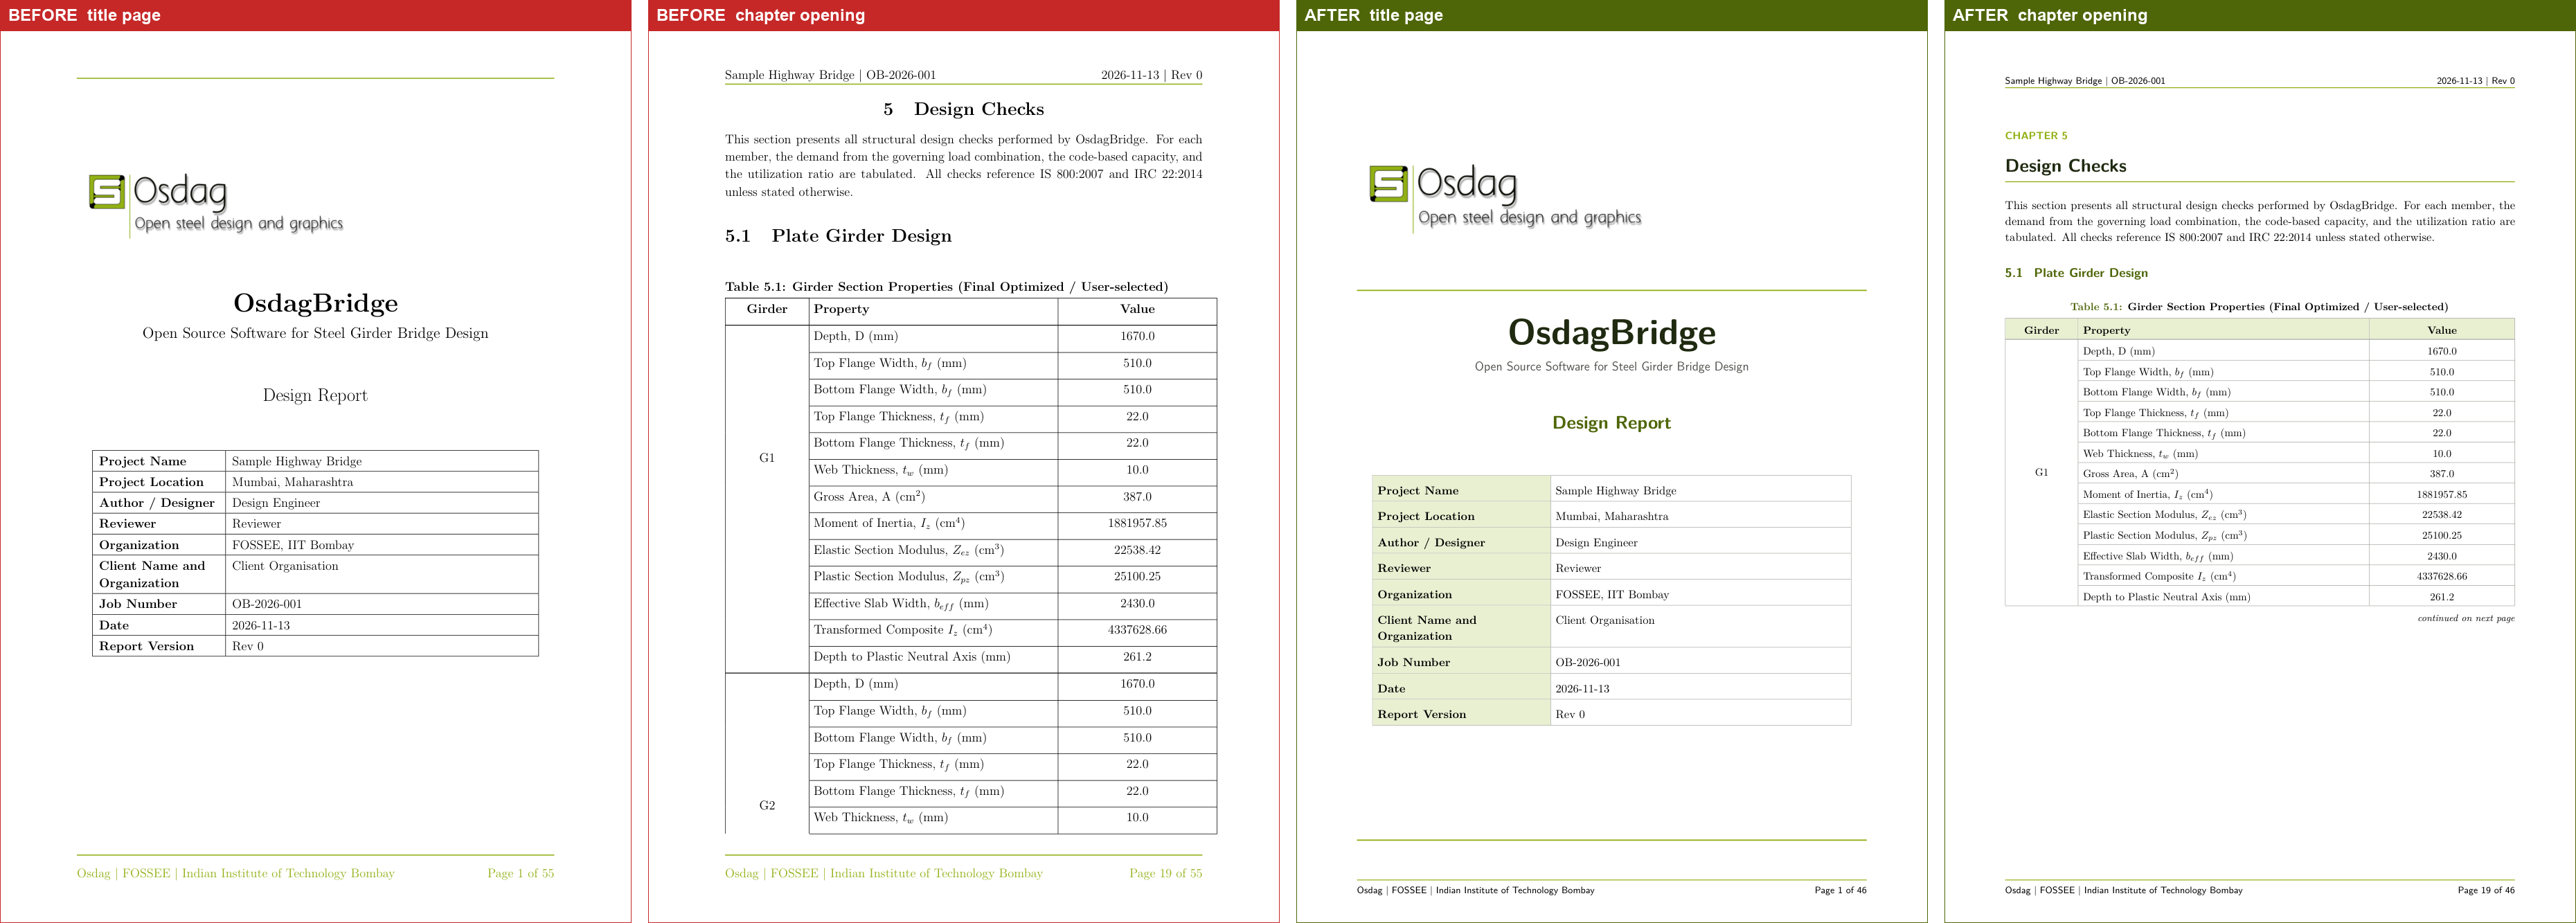
\includegraphics[width=\linewidth]{images/cmp_style.png}
\caption{Title page and chapter opening before and after the style system.}
\end{figure}

\section{Verification}
\begin{itemize}
\item \code{tools/report\_preview.py} runs one design headlessly, saves the results, and renders reports from that
snapshot with either source tree, so \emph{Report\_Before} and \emph{Report\_After} use identical design data.
\item Every page of both reports was rendered and inspected; LaTeX logs checked for errors and overfull boxes.
\item \code{pyflakes} on all report modules: no undefined names.
\item The submitted Report\_Before / Report\_After PDFs are produced from the desktop application
(Design $\rightarrow$ Generate Report) on the \code{dev} and \code{report-refactor} branches respectively, so they include the CAD views.
\end{itemize}

\section{Known limitations}
\begin{itemize}
\item The wheeled Class 70R/AA impact factor comes from the existing IRC~6 Cl.~208.3 impact-factor function, which
does not distinguish wheeled from tracked vehicles (it returns 1.10 at 30\,m); left unchanged as it is design logic.
\item End-diaphragm member forces are not returned by the current analysis, so their capacity checks show ``not evaluated''.
\item CAD views are captured from live GUI widgets, so the headless preview shows figure placeholders.
\end{itemize}

\end{document}
